\begin{chapter}{Funciones de Prueba}

\section*{ZDT (Zitzler-Deb-Thiele)} 

\textbf{Formulaci\'on de ZDT1:}

\begin{align*}
f_1(x)&=x_1\\
f_2(x,g(x))&=g(x)\cdot\left(1-\sqrt{ \frac{f_1}{g(x)}}\right)\\
g(x)&=1+\frac{9}{n-1}\cdot\sum_{i=2}^nx_i
\end{align*}

donde $n=30$ y $x_i\in[0,1]$ con $i=1,\ldots, n$. El \textit{frente de Pareto real} ($\mathcal{F}_{real}$) se forma con $g(x)=1$ y se muestra
en la figura \ref{fig:ZDT1}. Tiene un \textit{frente de Pareto} convexo.

\begin{figure}[h!]
 \centering
    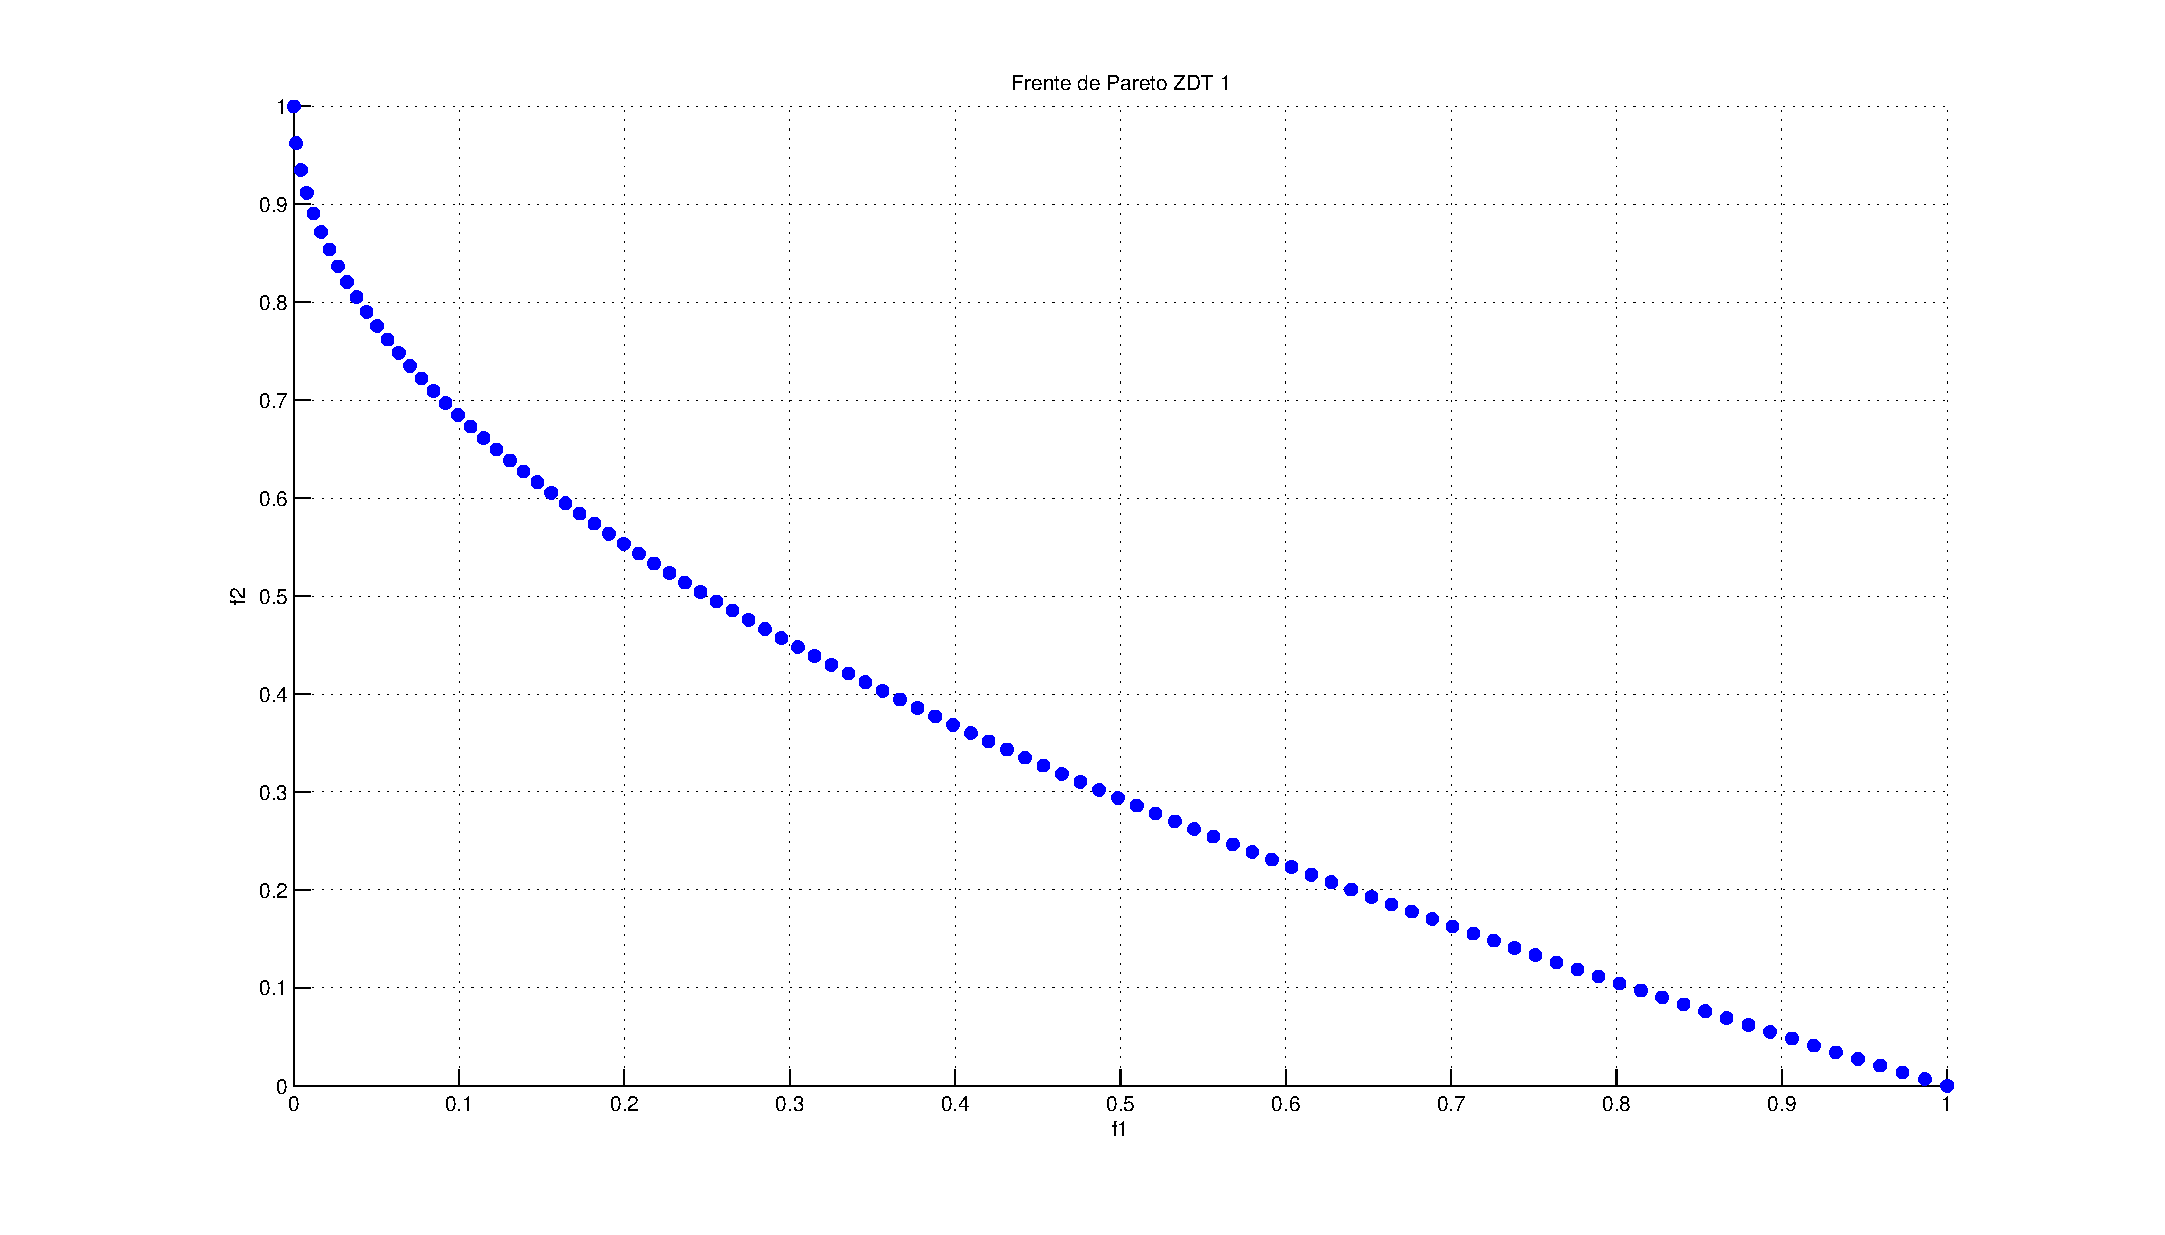
\includegraphics[scale=0.43]{ApendiceA/paretoZDT1.eps}
\caption{Frente de Pareto ZDT1}
\label{fig:ZDT1}
\end{figure} 

\textbf{Formulaci\'on de ZDT2:}

\begin{align*}
f_1(x)&=x_1\\
f_2(x,g(x))&=g(x)\cdot(1- \left( \frac{f_1}{g(x)}\right)^2)\\
g(x)&=1+\frac{9}{n-1}\cdot\sum_{i=2}^nx_i
\end{align*}

donde $n=30$ y $x_i\in[0,1]$ con $i=1,\ldots, n$. El \textit{frente de Pareto real} ($\mathcal{F}_{real}$) se forma con $g(x)=1$ y se muestra 
en la figura \ref{fig:ZDT2}. Tiene un \textit{frente de Pareto} c\'oncavo.

\begin{figure}[h!]
 \centering
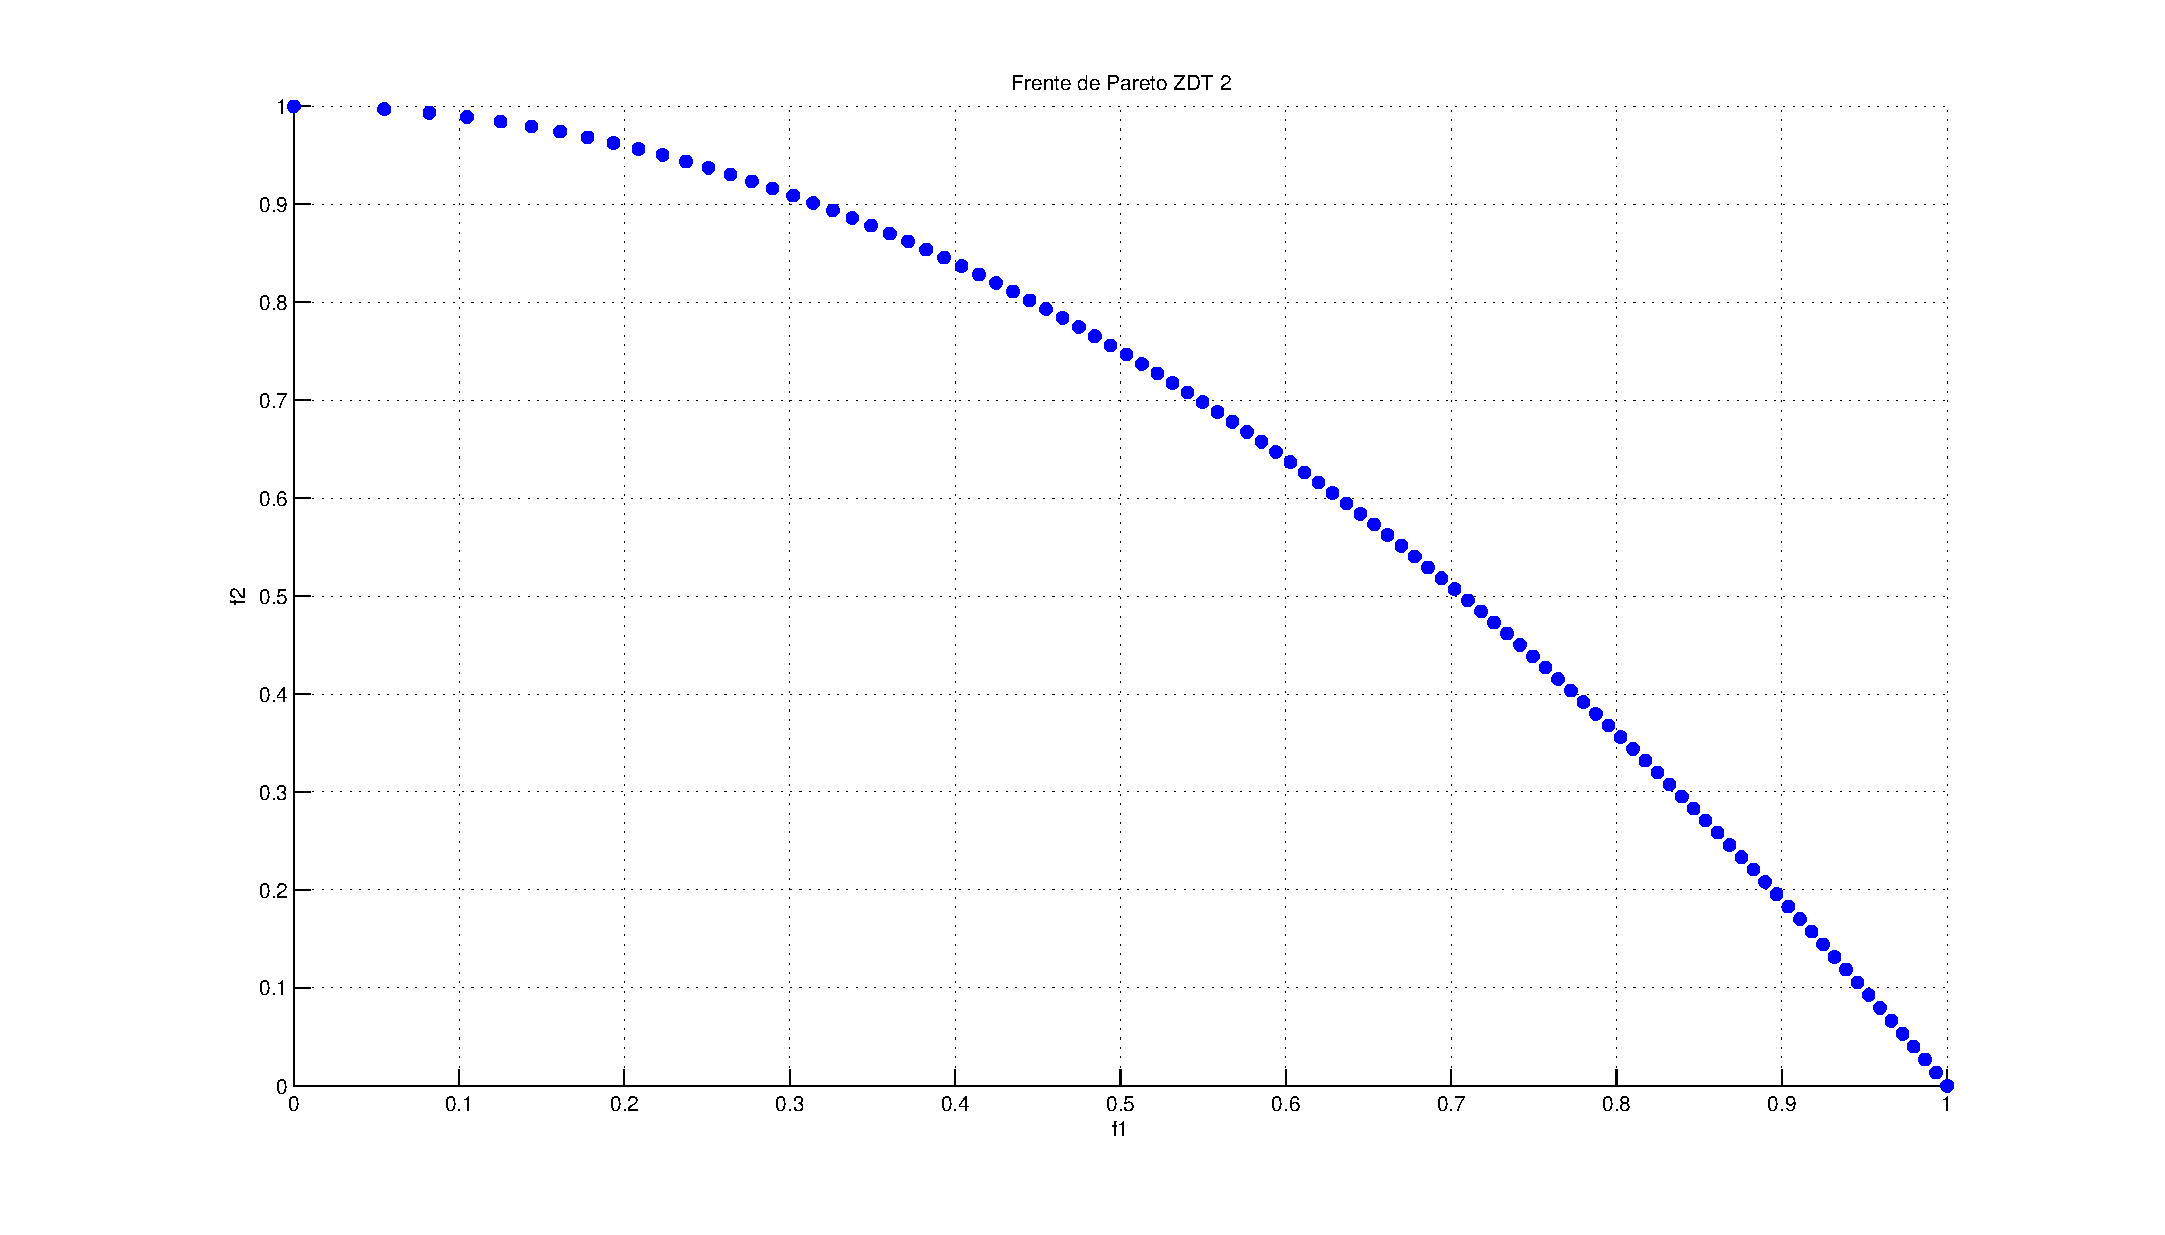
\includegraphics[scale=0.45]{ApendiceA/paretoZDT2.eps}
\caption{Frente de Pareto ZDT2}
\label{fig:ZDT2}
\end{figure} 

\textbf{Forumulaci\'on de ZDT3:}

\begin{align*}
f_1(x)&=x_1,\\
f_2(x,g)&=g(x)\cdot\left(1-\sqrt{\frac{f_1(x)}{g(x)}}-\frac{f_1(x)}{g(x)}\sin(10\cdot\pi\cdot f_1(x))\right)\\
g(x)&=1+\frac{9}{n-1}\cdot\sum_{i=2}^nx_i
\end{align*}

donde $n=30$ y $x_i\in[0,1]$ con $i=1, \ldots, n$. El \textit{frente de Pareto real} ($\mathcal{F}_{real}$) se forma con $g(x)=1$ y se muestra 
en la figura \ref{fig:ZDT3}. Tiene un {\it frente de Pareto} discontinuo y convexo.

\begin{figure}[h!]
 \centering
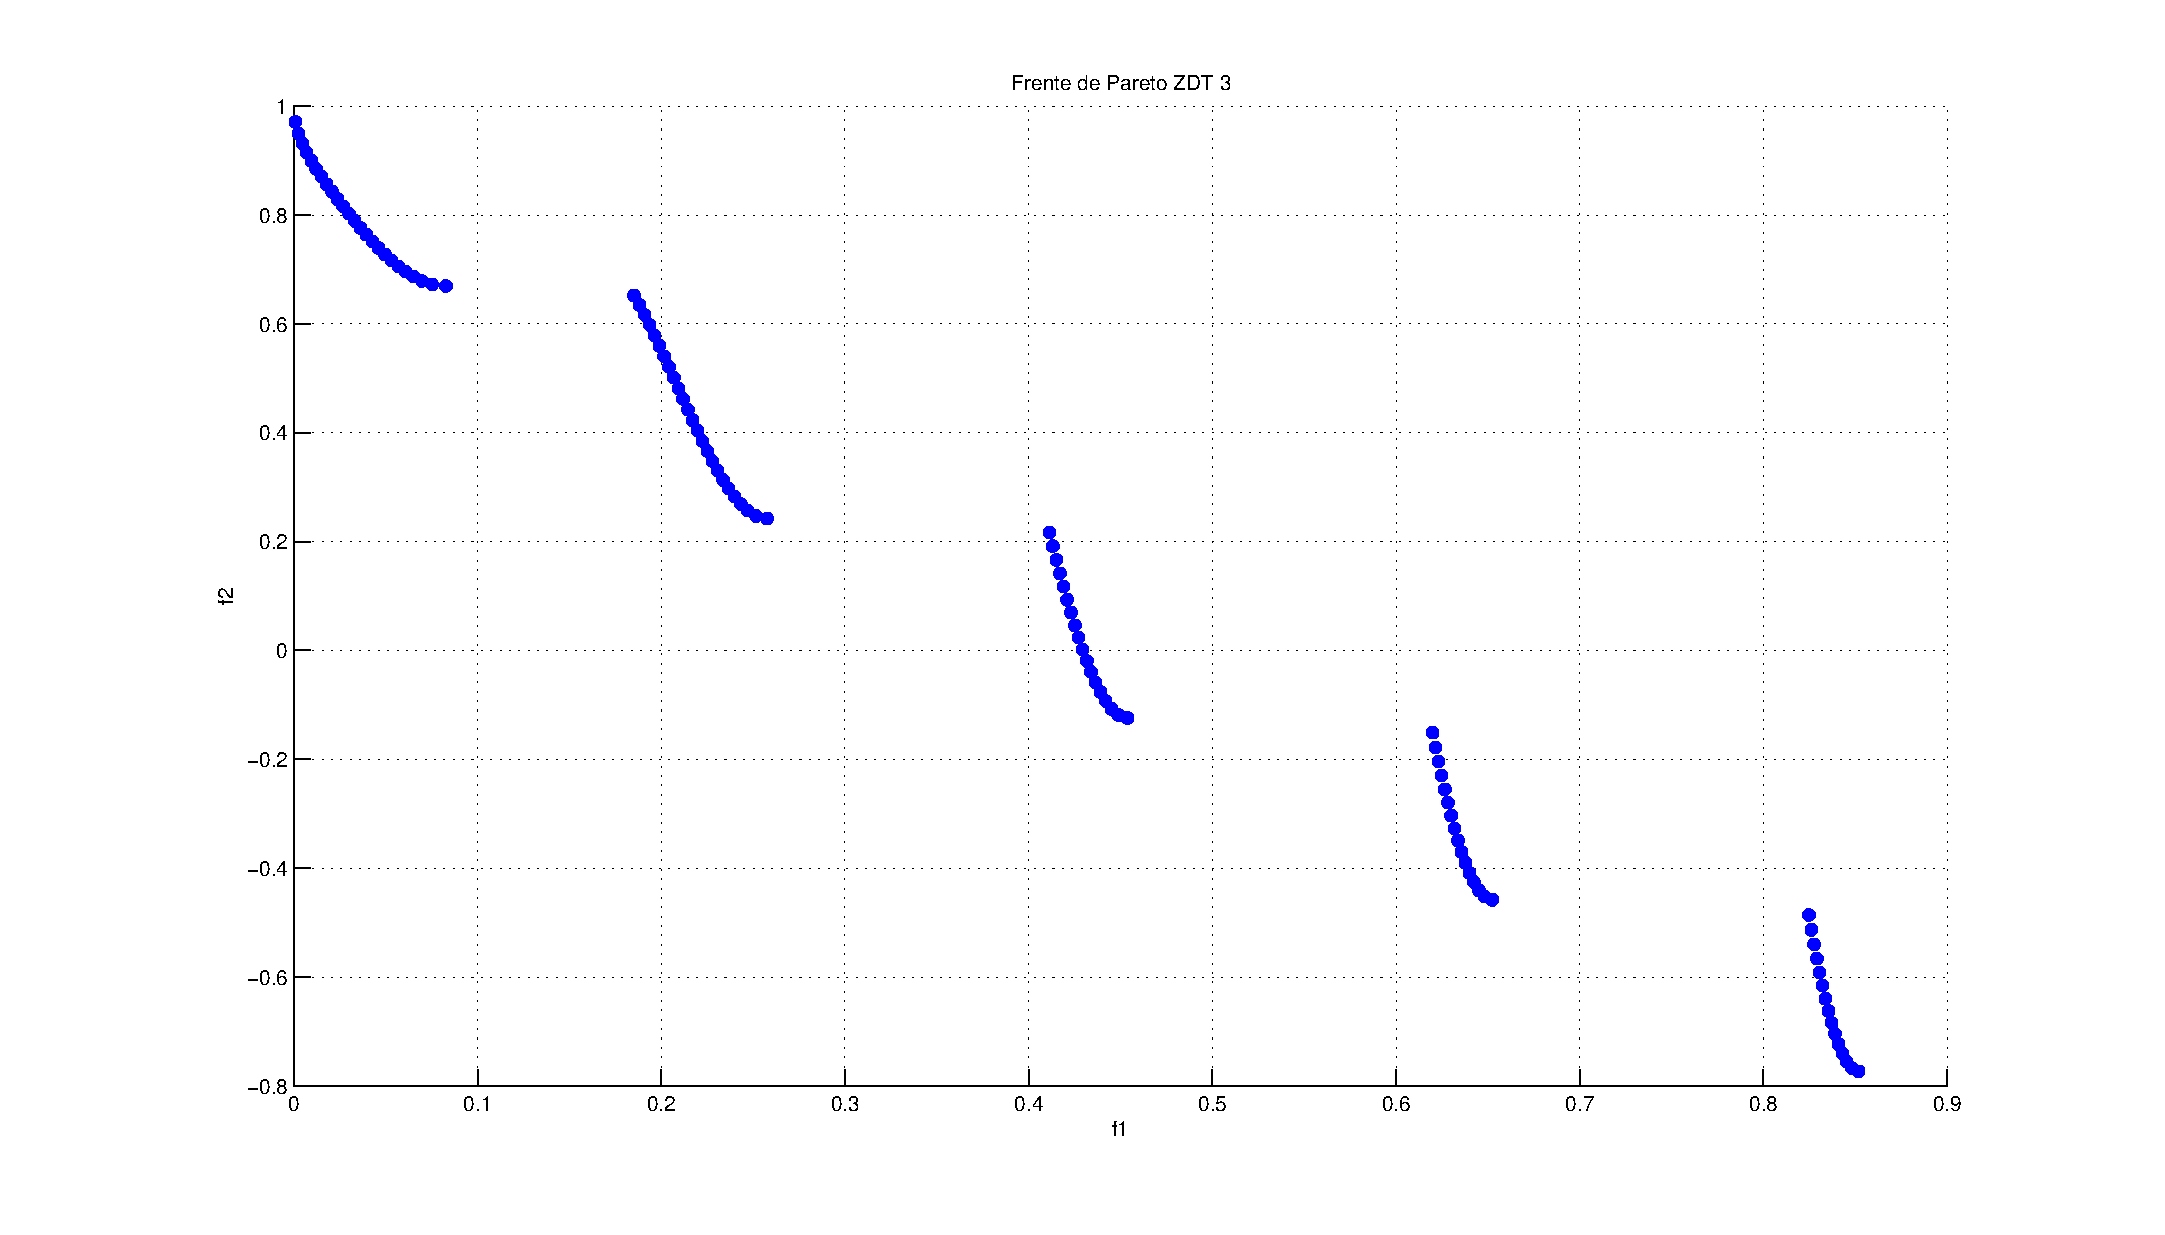
\includegraphics[scale=0.45]{ApendiceA/paretoZDT3.eps}
\caption{Frente de Pareto ZDT3}
\label{fig:ZDT3}
\end{figure} 

\textbf{Forumulaci\'on de ZDT4:}

\begin{align*}
f_1(x)&=x_1,\\
f_2(x,g(x))&=g(x)\cdot \left(1-\sqrt{ \frac{f_1(x)}{g(x)}}\right),\\
g(x)&=1+10\cdot(n-1)+ \sum_{i=2}^n(x_i^2-10\cdot \cos(4\cdot\pi\cdot x_i))
\end{align*}

donde $n=10$, $x_1\in[0,1]$ y $x_i \in[-5,5] $ con $i=2, \ldots, n$. El \textit{frente de Pareto real} ($\mathcal{F}_{real}$) se forma con $g(x)=1$ 
y se muestra en la figura \ref{fig:ZDT4}. Este problema tiene  $21^9$ frentes locales, lo que pone a prueba la habilidad de los algoritmos
evolutivos multi-objetivo de lidiar con problemas multifrontales.

\begin{figure}[h!]
 \centering
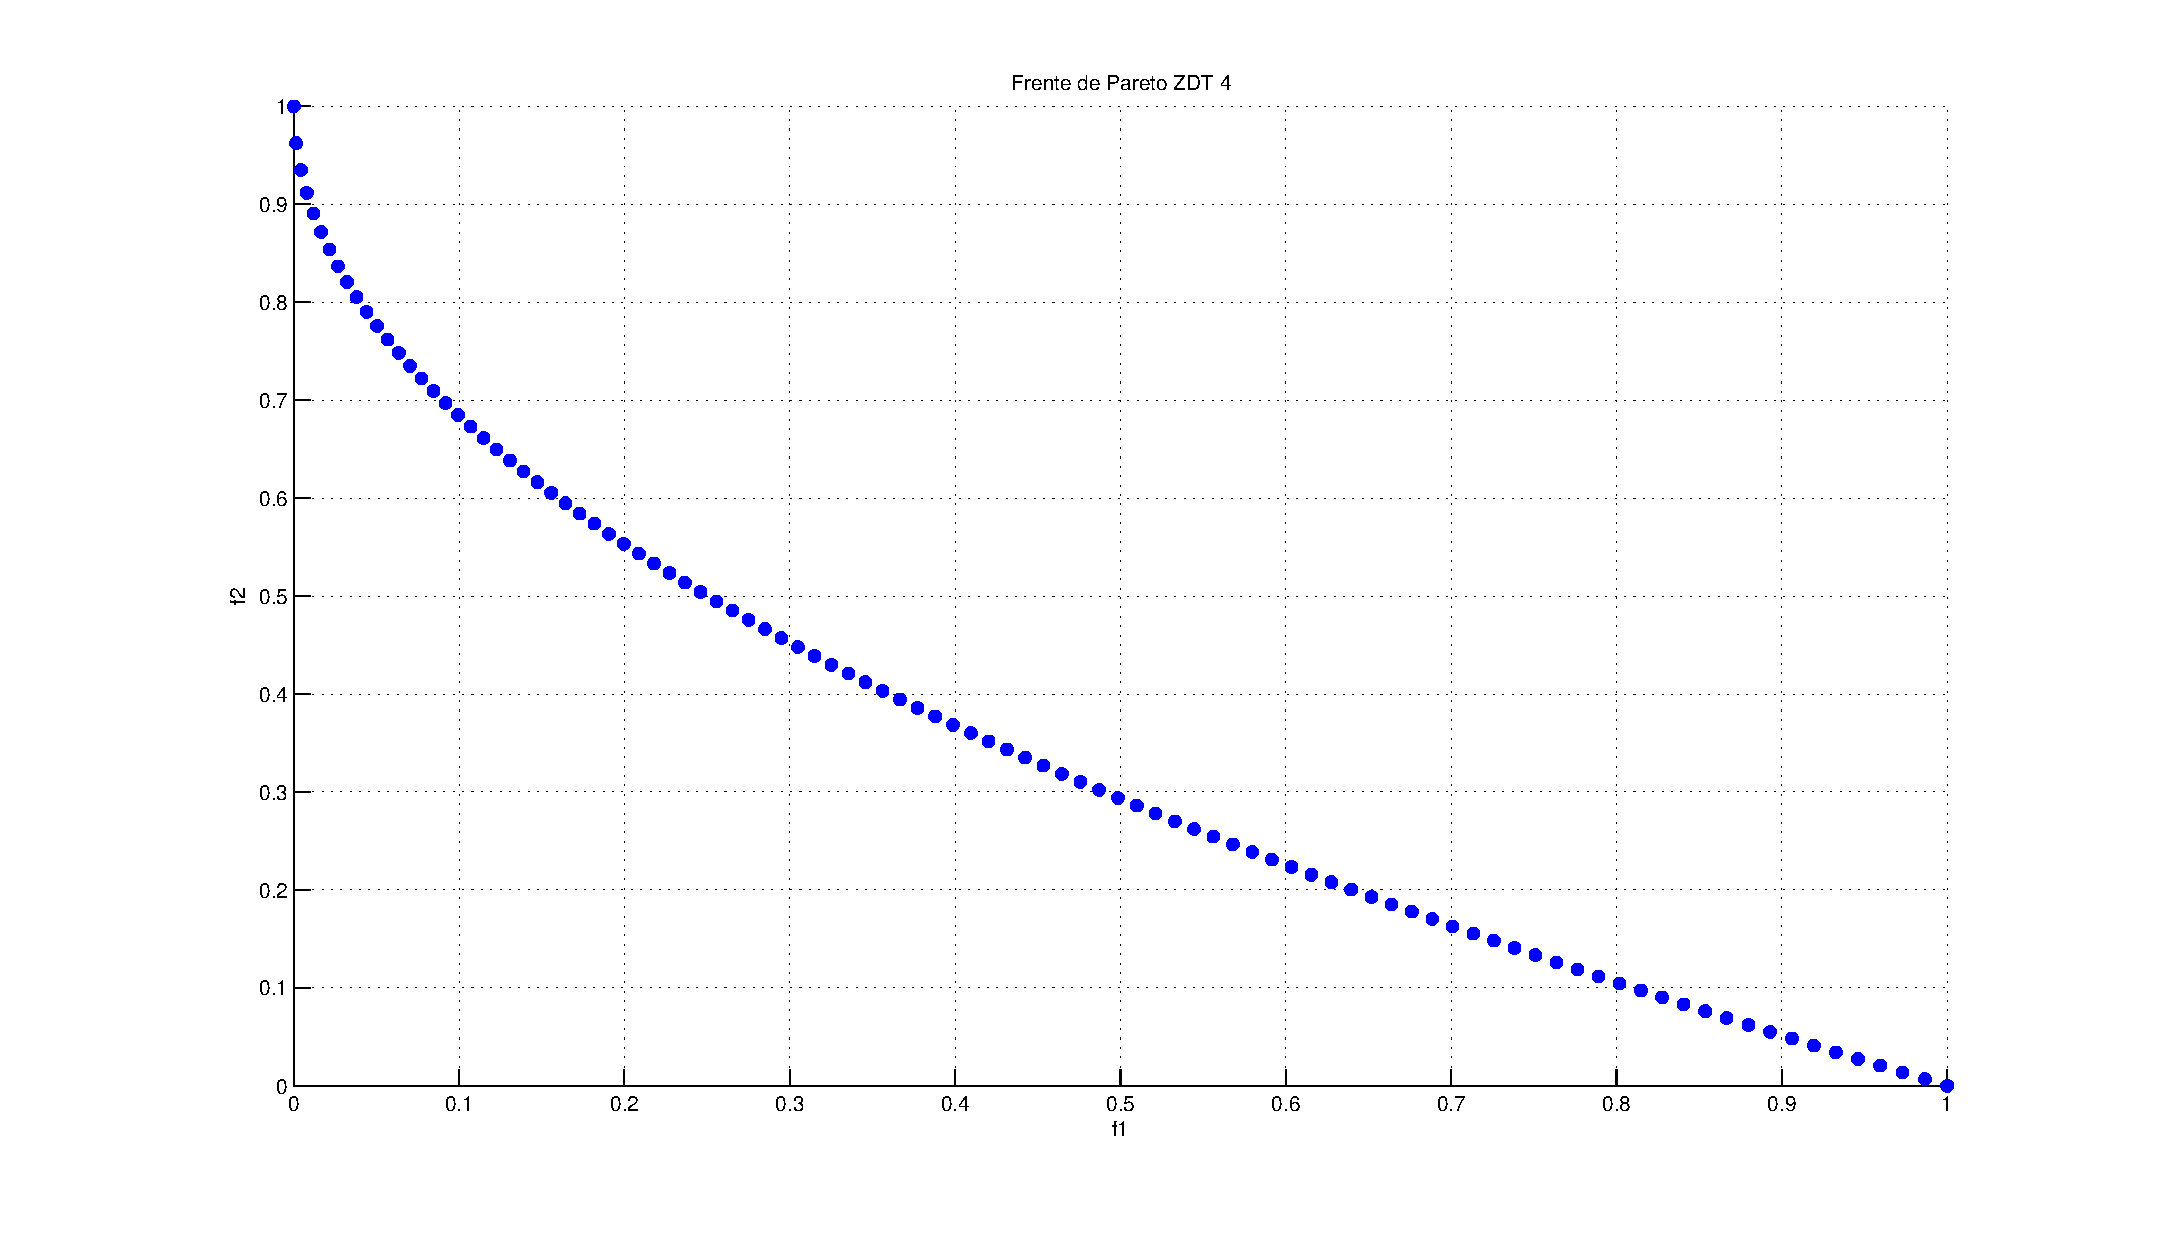
\includegraphics[scale=0.45]{ApendiceA/paretoZDT4.eps}
\caption{Frente de Pareto ZDT4}
\label{fig:ZDT4}
\end{figure} 

\textbf{Formulaci\'on de ZDT6:}

\begin{align*}
f_1(x)&=1- e^{(-4\cdot x_1)} \cdot \sin^6(6\cdot\pi\cdot x_1),\\
f_2(x,g(x))&=g(x)\cdot(1-\left(\frac{f_1}{g(x)}\right)^2),\\
g(x)&=1+9\cdot\left[\frac{\sum_{i=2}^n}{9}\right]^{0.25}
\end{align*}

donde $n=10$, $x_1\in[0,1]$ y $x_i \in[-5,5]$ con $i= 2, \ldots, n$. El \textit{frente de Pareto real} ($\mathcal{F}_{real}$) se forma con $g(x)=1$
y se muestra en la figura \ref{fig:ZDT6}. El espacio de b\'usqueda no es uniforme, tiene una baja densidad en las soluciones cerca del 
$\mathcal{F}_{real}$ y una alta densidad lejos del mismo.

\begin{figure}[h!]
 \centering
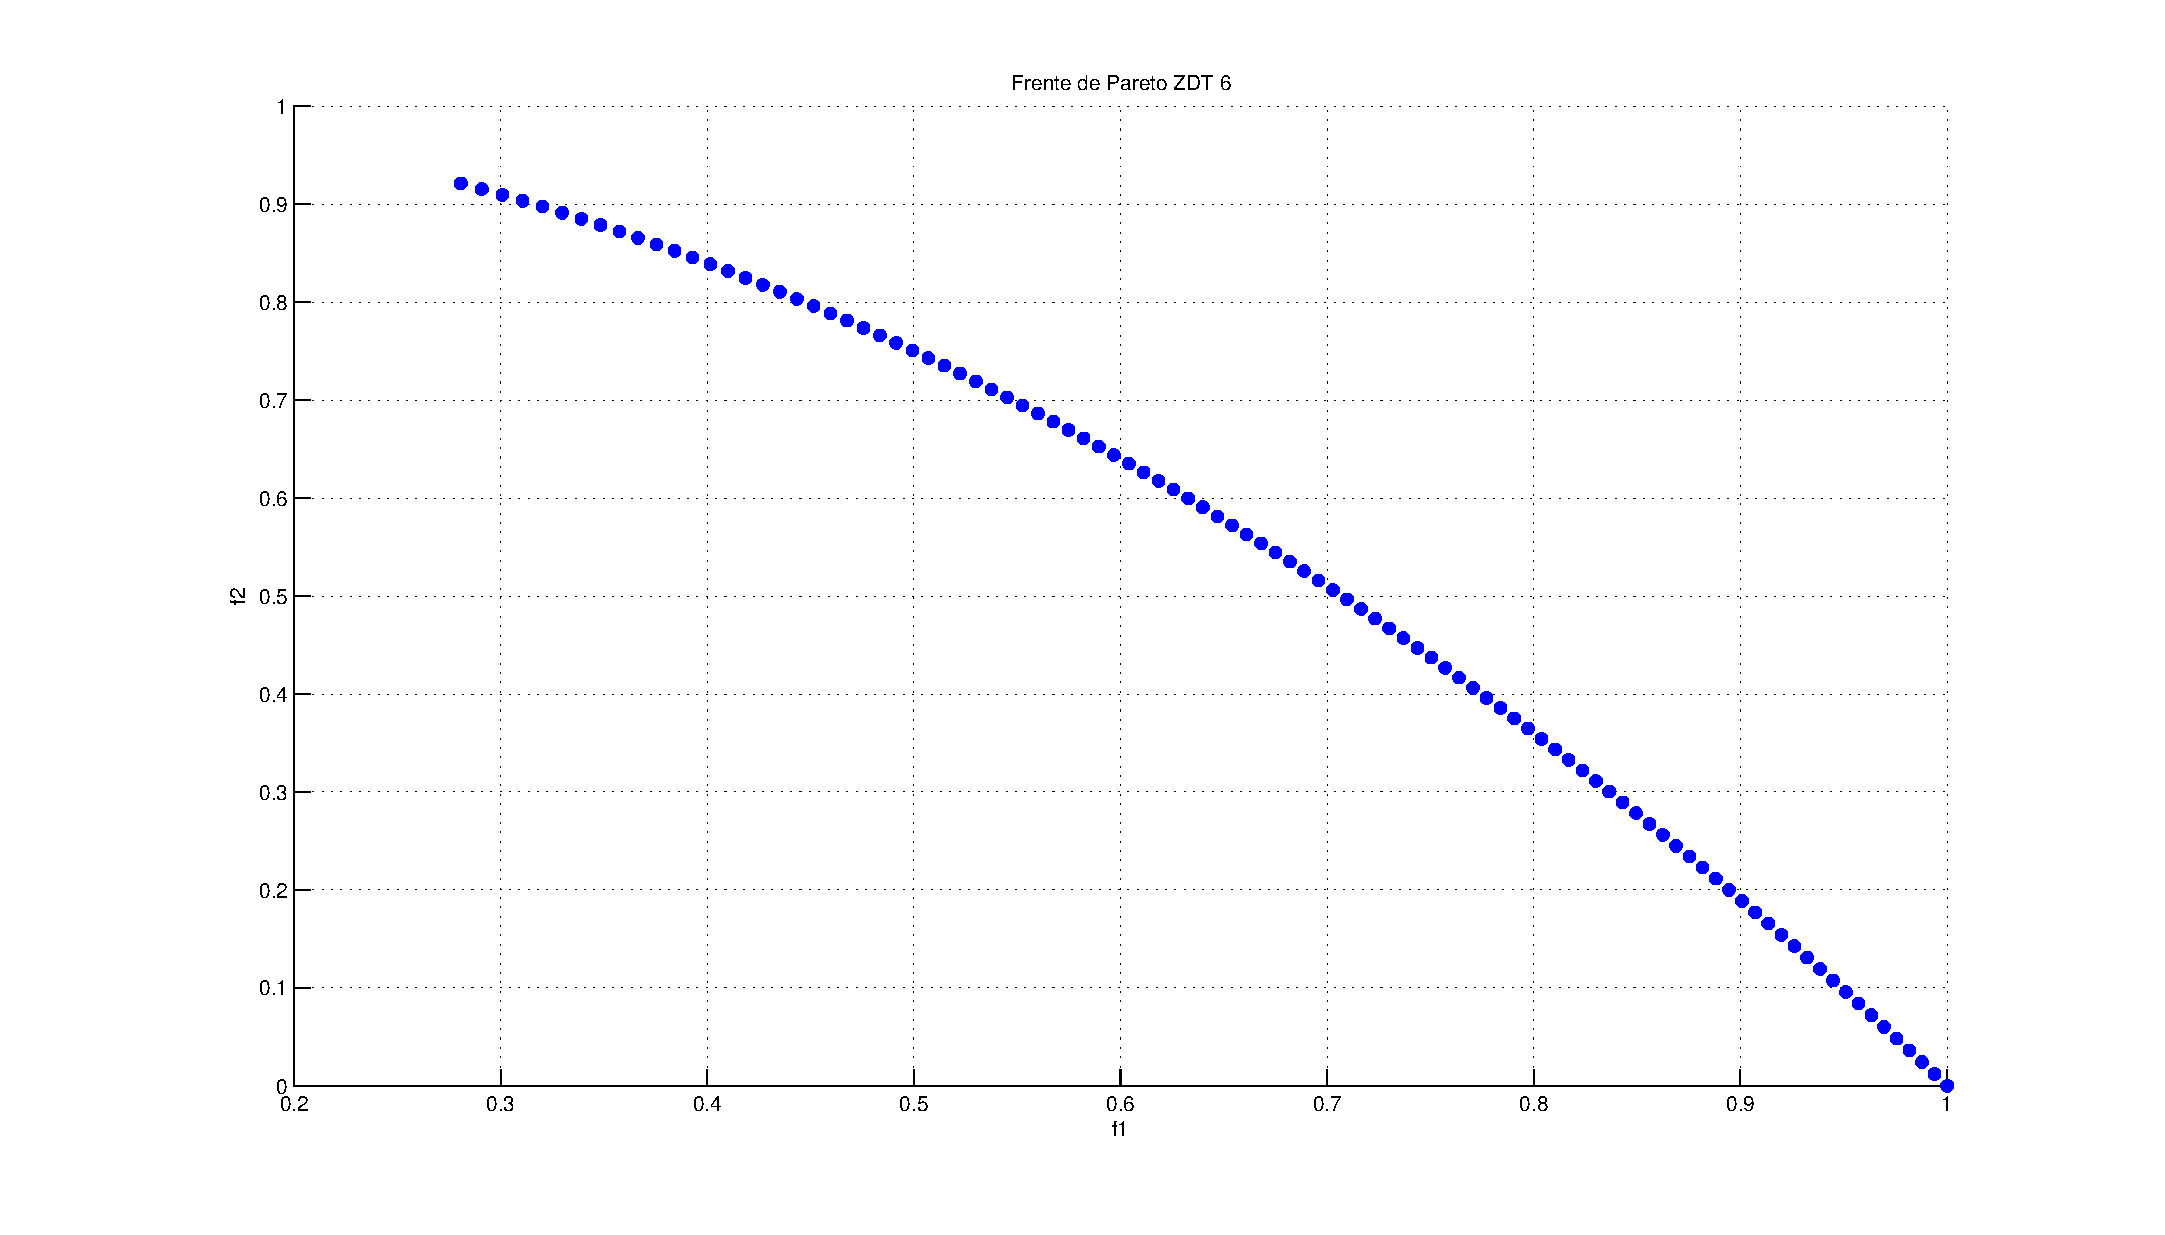
\includegraphics[scale=0.45]{ApendiceA/paretoZDT6.eps}
\caption{Frente de Pareto ZDT6}
\label{fig:ZDT6}
\end{figure} 

\section*{DTLZ (Deb-Thiele-Laumanns-Zitzler)} 

\textbf{Formulaci\'on de DTLZ1:}

\begin{align*}
f_1(x)&=\frac{1}{2}\cdot x_1\cdot x_2 \cdot \ldots \cdot x_{M-1} \cdot (1+g(x))\\
f_2(x)&=\frac{1}{2}\cdot x_1\cdot x_2 \cdot \ldots \cdot(1-x_{M-1})\cdot(1+g(x))\\
\vdots&\\
f_M(x)&=\frac{1}{2}\cdot(1-x_1)\cdot(1+g(x))\\
g(x)&=100\cdot[k+\sum_{i=M}^n(x_i-0.5)^2-cos(20\cdot\pi\cdot(x_i-0.5))]
\end{align*}

donde $n=M+k-1$ (se sugiere un $k=5$) y $x_i\in[0,1]$ con $i = 1, \ldots, n$. El \textit{frente de Pareto real} ($\mathcal{F}_{real}$) para $M=3$ se muestra
en la figura \ref{fig:DTLZ1}. Este problema tiene un {\it frente de Pareto}  lineal, separable y multimodal. El espacio de b\'usqueda 
contiene $11^k-1$ frentes locales. 

\begin{figure}[h!]
 \centering
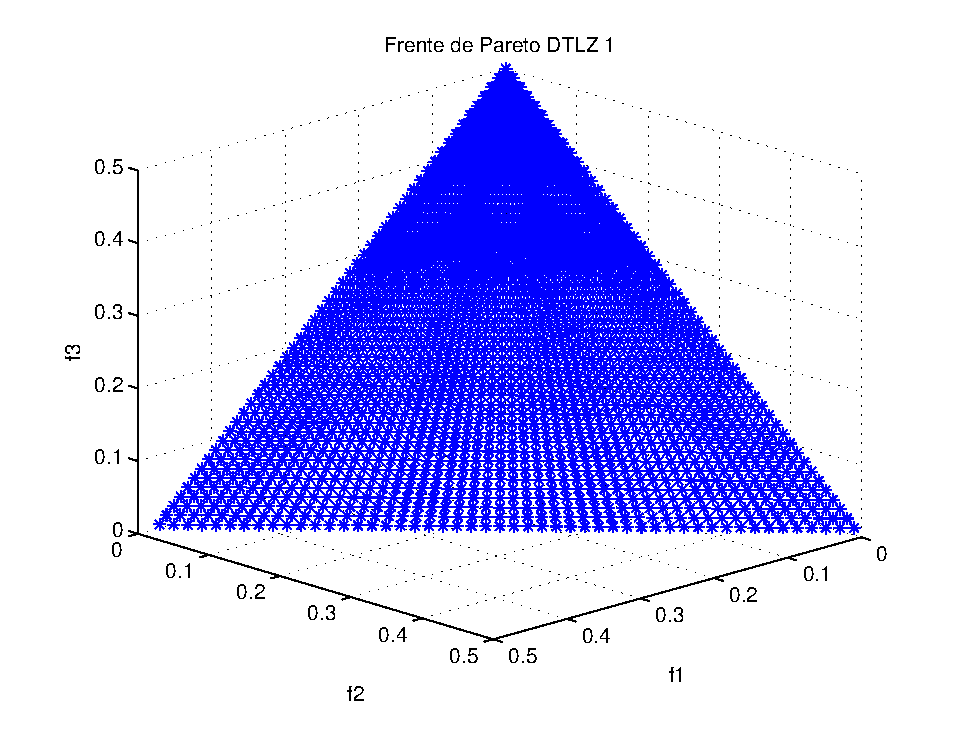
\includegraphics[scale=0.4]{ApendiceA/paretoDTLZ1.eps}
\caption{Frente de Pareto DTLZ1}
\label{fig:DTLZ1}
\end{figure}

\textbf{Formulaci\'on de DTLZ2:}

\begin{align*}
f_1(x)&=\cos(x_1\frac{\pi}{2})\cdot\cos(x_2\frac{\pi}{2})\cdot\ldots\cdot\cos(x_{M-1}\frac{\pi}{2})\cdot(1+g(x))\\
f_2(x)&=\cos(x_1\frac{\pi}{2})\cdot\cos(x_2\frac{\pi}{2})\cdot\ldots\cdot\sin(x_{M-1}\frac{\pi}{2})\cdot(1+g(x))\\
f_3(x)&=\cos(x_1\frac{\pi}{2})\cdot\cos(x_2\frac{\pi}{2})\cdot\ldots\cdot\sin(x_{M-2}\frac{\pi}{2})\cdot(1+g(x))\\
\vdots&\\
f_{M-1}(x)&=\cos(x_1\frac{\pi}{2})\cdot\sin(x_2\frac{\pi}{2})(1+g(x))\\
f_{M}(x)&=\sin(x_1\frac{\pi}{2})\cdot(1+g(x))\\
g(x)&=\sum_i=(x_i-0.5)^2
\end{align*}

donde $n=M+k-1$ (se sugiere un $k=10$) y $x_i\in[0,1]$ con $i= 1, \ldots, n$. El \textit{frente de Pareto real} ($\mathcal{F}_{real}$)
para $M=3$ se muestra en la figura \ref{fig:DTLZ2}. Tiene un {\it frente de Pareto}  c\'oncavo. Este problea se puede utilizar para 
investigar la habilidad de escalabilidad en objetivos de un algoritmo evolutivo multi-objetivo.

\begin{figure}[h!]
 \centering
\includegraphics[scale=0.4]{ApendiceA/paretoDTLZ2.eps}
\caption{Frente de Pareto DTLZ2}
\label{fig:DTLZ2}
\end{figure}

\textbf{Formulaci\'on de DTLZ3}

\begin{align*}
f_1(x)&=\cos(x_1\frac{\pi}{2})\cdot\cos(x_2\frac{\pi}{2})\cdot\ldots\cdot \cos(x_{M-1}\frac{\pi}{2})\cdot(1+g(x))\\
f_2(x)&=\cos(x_1\frac{\pi}{2})\cdot\cos(x_2\frac{\pi}{2})\cdot\ldots\cdot \sin(x_{M-1}\frac{\pi}{2})\cdot(1+g(x))\\
f_3(x)&=\cos(x_1\frac{\pi}{2})\cdot\cos(x_2\frac{\pi}{2})\cdot\ldots\cdot \sin(x_{M-2}\frac{\pi}{2})\cdot(1+g(x))\\
\vdots&\\
f_{M-1}(x)&=\cos(x_1\frac{\pi}{2})\cdot\sin(x_2\frac{\pi}{2})\cdot(1+g(x))\\
f_{M}(x)&=\sin(x_1\frac{\pi}{2})\cdot (1+g(x))\\
g(x)&=100\cdot [k+\sum_{i=M}^n(x_i-0.5)^2-\cos(20\cdot\pi\cdot(x_i-0.5))]
\end{align*}


donde $n=M+k-1$ (se sugiere un $k=10$) y $x_i\in[0,1]$ con $i=1, \ldots, n$. La funci\'on $g(x)$ introduce  $3\cdot k-1$ frentes locales 
paralelos al frente global. El \textit{frente de Pareto real} ($\mathcal{F}_{real}$) para $M=3$ se muestra en la figura \ref{fig:DTLZ3}.
Tiene un {\it frente de Pareto}  c\'oncavo y multimodal. Este problema prueba la habilidad de un algoritmo evolutivo multi-objetivo de converger al 
$\mathcal{F}_{real}$.

\begin{figure}[h!]
 \centering
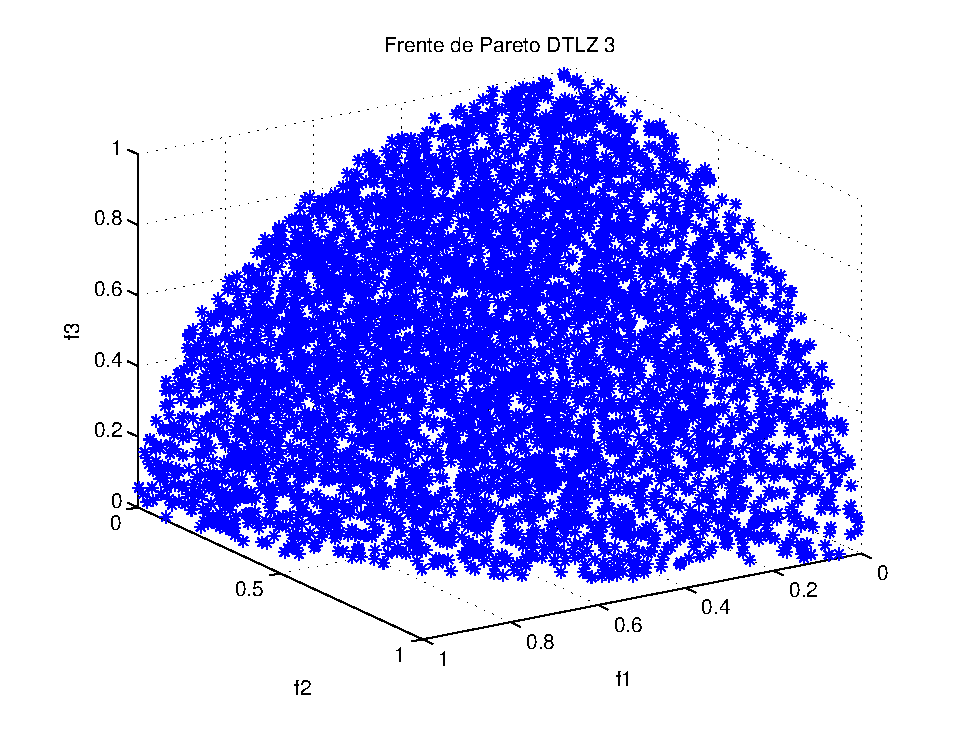
\includegraphics[scale=0.4]{ApendiceA/paretoDTLZ3.eps}
\caption{Frente de Pareto DTLZ3}
\label{fig:DTLZ3}
\end{figure}

\textbf{Formulaci\'on de DTLZ4}

\begin{align*}
f_1(x)&=\cos(x_1^\alpha\frac{\pi}{2})\cdot\cos(x_2^\alpha\frac{\pi}{2})\cdot\ldots\cdot cos(x_{M-1}^\alpha\frac{\pi}{2})\cdot(1+g(x))\\
f_2(x)&=\cos(x_1^\alpha\frac{\pi}{2})\cdot\cos(x_2^\alpha\frac{\pi}{2})\cdot\ldots\cdot sin(x_{M-1}^\alpha\frac{\pi}{2})\cdot(1+g(x))\\
f_3(x)&=\cos(x_1^\alpha\frac{\pi}{2})\cdot\cos(x_2^\alpha\frac{\pi}{2})\cdot\ldots\cdot sin(x_{M-2}^\alpha\frac{\pi}{2})\cdot(1+g(x))\\
\vdots&\\
f_{M-1}(x)&=\cos(x_1^\alpha\frac{\pi}{2})\cdot\sin(x_2^\alpha\frac{\pi}{2})\cdot(1+g(x))\\
f_{M}(x)&=\sin(x_1^\alpha\frac{\pi}{2})\cdot(1+g(x))\\
g(x)&=\sum_i(x_i-0.5)^2
\end{align*}


donde $n=M+k-1$ (se sugiere $k=10$ y $\alpha=100$) y $x_i\in[0,1]$ con $i=1,\ldots, n$. El \textit{frente de Pareto real} ($\mathcal{F}_{real}$) 
para $M=3$ se muestra en la figura \ref{fig:DTLZ4}. Tiene un {\it frente de Pareto}  c\'oncavo, separable y multimodal. Este probema prueba 
la habilidad de los algoritmos evolutivos multi-objetivo de mantener una buena distribuci\'on de las soluciones.

\begin{figure}[h!]
 \centering
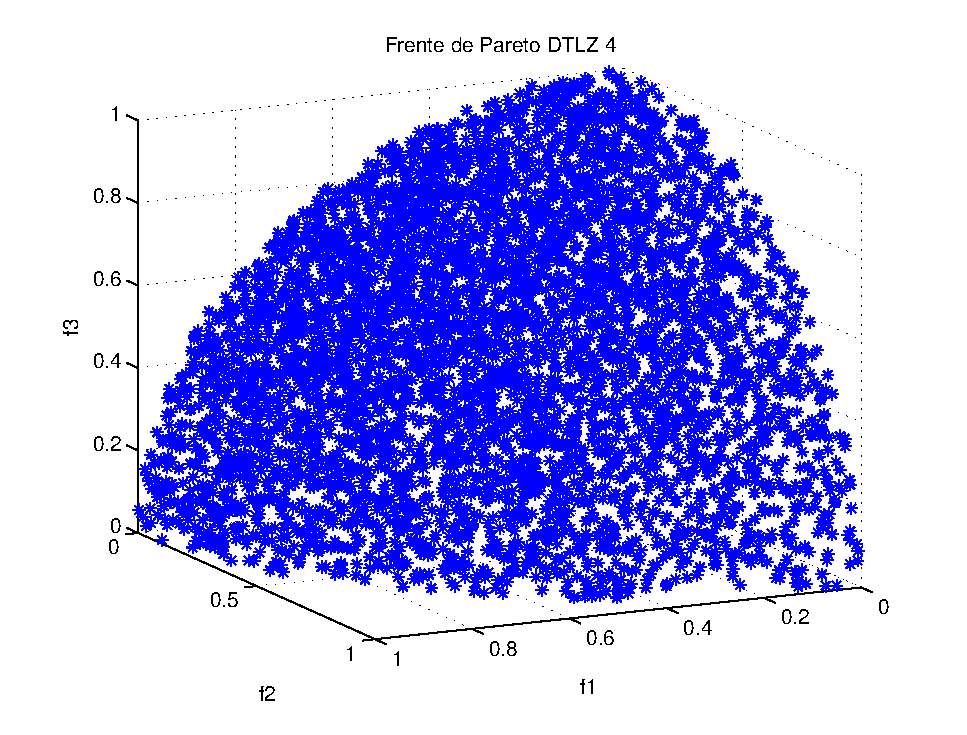
\includegraphics[scale=0.4]{ApendiceA/paretoDTLZ4.eps}
\caption{Frente de Pareto DTLZ4}
\label{fig:DTLZ4}
\end{figure}

\textbf{Formulaci\'on de DTLZ5}

\begin{align*}
f_1(x)&=\cos(\theta_1\frac{\pi}{2})\cdot\cos(\theta_2\frac{\pi}{2})\cdot\ldots\cdot \cos(\theta_{M-1}\frac{\pi}{2})\cdot(1+g(x))\\
f_2(x)&=\cos(\theta_1\frac{\pi}{2})\cdot\cos(\theta_2\frac{\pi}{2})\cdot\ldots\cdot \sin(\theta_{M-1}\frac{\pi}{2})\cdot(1+g(x))\\
f_3(x)&=\cos(\theta_1\frac{\pi}{2})\cdot\cos(\theta_2\frac{\pi}{2})\cdot\ldots\cdot \sin(\theta_{M-2}\frac{\pi}{2})\cdot(1+g(x))\\
\vdots&\\
f_{M-1}(x)&=\cos(\theta_1\frac{\pi}{2})\cdot\sin(\theta_2\frac{\pi}{2})\cdot(1+g(x))\\
f_{M}(x)&=\sin(\theta_1\frac{\pi}{2})\cdot(1+g(x))\\
\theta_1&=\frac{\pi}{2}x_1\\
\theta_i&=\frac{\pi}{4\cdot(1+g(x))}(1+2\cdot g(x)\cdot x_i),  \text{para} \hspace{1mm} i=2,3\dots,(M-1)\\
g(x)&=\sum^n_i(x_i-0.5)^2
\end{align*}

donde $n=M+k-1$ (se sugiere un $k=10$) y $x_i\in[0,1]$ con $i = 1,\ldots,n$. El \textit{frente de Pareto real} ($\mathcal{F}_{real}$) 
para $M=3$ se muestra en la figura \ref{fig:DTLZ5}. Este problema tiene un {\it frente de Pareto} curvo.

\begin{figure}[h!]
 \centering
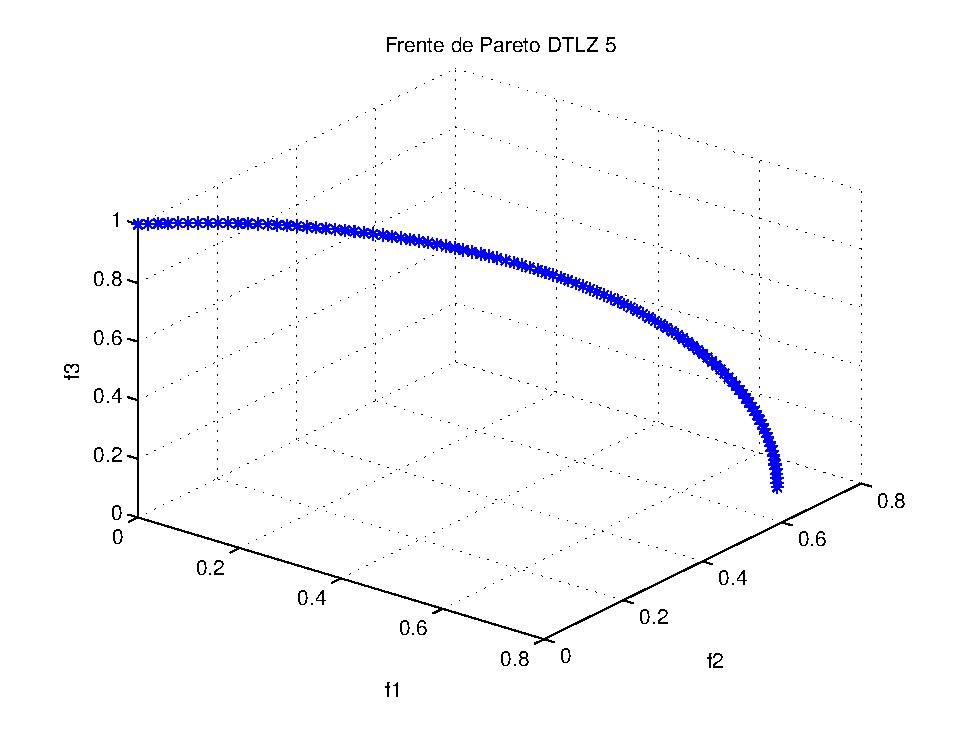
\includegraphics[scale=0.4]{ApendiceA/paretoDTLZ5.eps}
\caption{Frente de Pareto DTLZ5}
\label{fig:DTLZ5}
\end{figure}

\textbf{Formulaci\'on de DTLZ6}

\begin{align*}
f_1(x)&=\cos(\theta_1\frac{\pi}{2})\cdot\cos(\theta_2\frac{\pi}{2})\cdot\ldots\cdot \cos(\theta_{M-1}\frac{\pi}{2})\cdot(1+g(x))\\
f_2(x)&=\cos(\theta_1\frac{\pi}{2})\cdot\cos(\theta_2\frac{\pi}{2})\cdot\ldots\cdot \sin(\theta_{M-1}\frac{\pi}{2})\cdot(1+g(x))\\
f_3(x)&=\cos(\theta_1\frac{\pi}{2})\cdot\cos(\theta_2\frac{\pi}{2})\cdot\ldots\cdot \sin(\theta_{M-2}\frac{\pi}{2})\cdot(1+g(x))\\
\vdots&\\
f_{M-1}(x)&=\cos(\theta_1\frac{\pi}{2})\cdot\sin(\theta_2\frac{\pi}{2})\cdot(1+g(x))\\
f_{M}(x)&=\sin(\theta_1\frac{\pi}{2})\cdot(1+g(x))\\
\theta_1&=\frac{\pi}{2}x_1\\
\theta_i&=\frac{\pi}{4(1+g(x))}(1+2\cdot g(x)\cdot x_i),  \text{para}\hspace{1mm} i=2,3\dots,(M-1)\\
g(x)&=\sum^n_i=(x_i-0.5)^0.1
\end{align*}

donde $n=M+k-1$ (se sugiere un $k=10$) y $x_i\in[0,1]$ con $i=1,\ldots,n$.  El \textit{frente de Pareto real} ($\mathcal{F}_{real}$) para 
$M=3$ se muestra en la figura \ref{fig:DTLZ6}. En este problema se modifica la funci\'on $g(x)$ de DTLZ5 volvi\'endolo m\'as dif\'icil. 
Tiene un {\it frente de Pareto} curvo.

\begin{figure}[h!]
 \centering
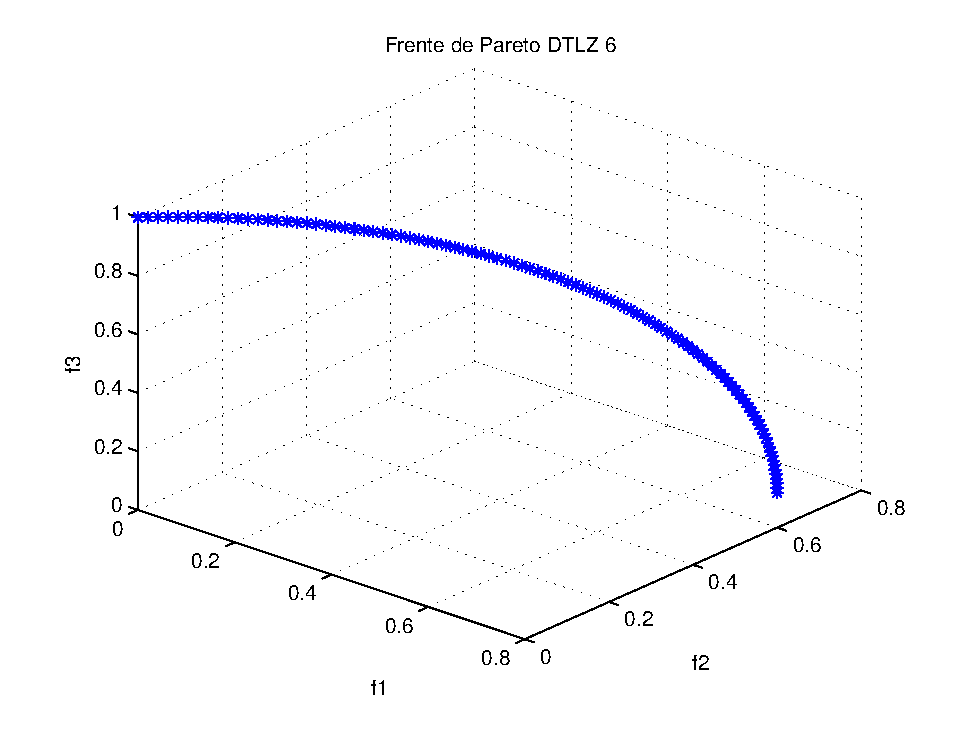
\includegraphics[scale=0.4]{ApendiceA/paretoDTLZ6.eps}
\caption{Frente de Pareto DTLZ6}
\label{fig:DTLZ6}
\end{figure}

\textbf{Formulaci\'on de DTLZ7}

\begin{align*}
f_1(x)&=x_1 \\
f_2(x)&=x_2\\
\vdots&\\
f_{M-1}(x)&=x_{M-1}\\
f_{M}(x)&=(1+g(x_M))\cdot h(f_1,f_2,\dots,f_{M-1}g(x))\\
g(x)&=1+\frac{9}{k}\cdot\sum_{i=2}^nx_i\\
h(f_1,f_2,\dots,f_{M-1}g(x))&=M-\sum_{i=1}^{M-1}(\frac{f_i}{1+g(x)}(1+\sin{(3\cdot\pi\cdot f_i)}))
\end{align*}


donde $n=M+k-1$ (se sugiere un $k=20$) y $x_i\in[0,1]$ con $i=1,\ldots,n$. El \textit{frente de Pareto real} ($\mathcal{F}_{real}$) para 
$M=3$ se muestra en la figura \ref{fig:DTLZ7}. Tiene un {\it frente de Pareto} discontinuo. Este problema prueba la habilidad de un \
algoritmo evolutivo multi-objetivo de mantener individuos en las diferentes regiones del {\it frente de Pareto}.

\begin{figure}[h!]
 \centering
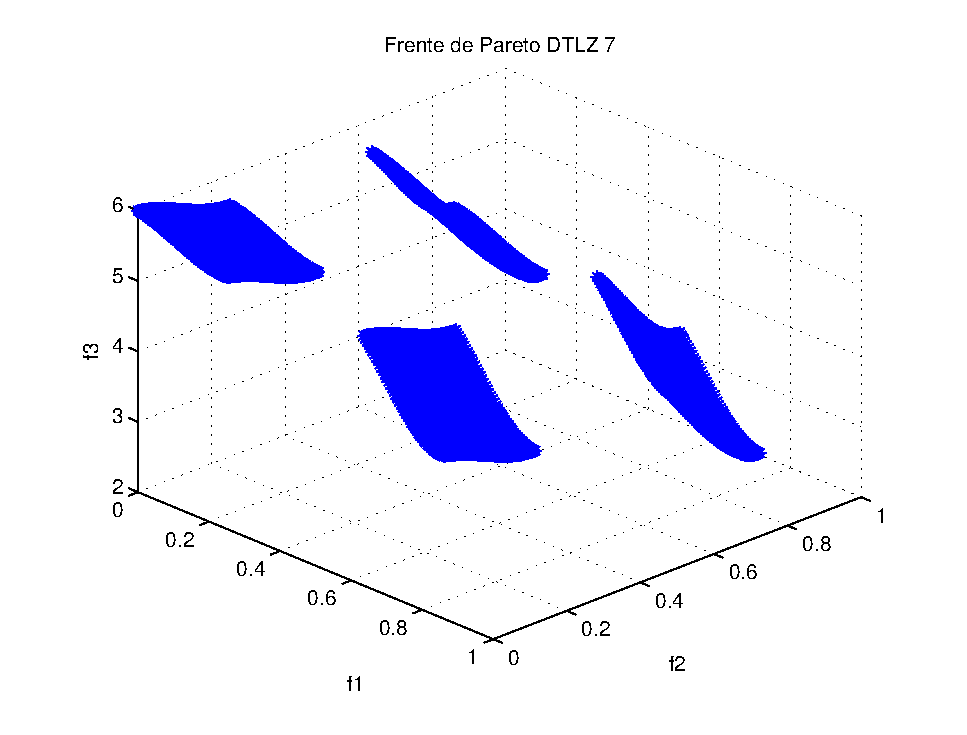
\includegraphics[scale=0.4]{ApendiceA/paretoDTLZ7.eps}
\caption{Frente de Pareto DTLZ7}
\label{fig:DTLZ7}
\end{figure}

\end{chapter}



















